\documentclass[notes]{subfiles}
\begin{document}
	\addcontentsline{toc}{section}{12.3 - The Dot Product}
	\refstepcounter{section}
	\fancyhead[RO,LE]{\bfseries \nameref{cs123}} 
	\fancyhead[LO,RE]{\bfseries \small \currentname}
	\fancyfoot[C]{{}}
	\fancyfoot[RO,LE]{\large \thepage}	%Footer on Right \thepage is pagenumber
	\fancyfoot[LO,RE]{\large Chapter 12.3}
	
\section*{The Dot Product}\label{cs123}
	\subsection*{Before Class}
	\subsubsection*{The Dot Product}
		\begin{defn}[Dot Product (Algebraic Definition)]
			If $\textbf{a} = \lrangle{a_1,a_2,a_3,\cdots, a_n}$ and $\textbf{b} =\lrangle{b_1,b_2,b_3,\cdots, b_n}$, then the \textbf{dot product} of \textbf{a} and \textbf{b} is given by\\[15pt]
				\[\textbf{a}\cdot\textbf{b} = \hspace{3in}\]
		\end{defn}
		
		\begin{ex}
			Let $\textbf{a} = \lrangle{1,0,1}$, $\textbf{b} = \lrangle{2,5,-3}$, and $\textbf{c} = \lrangle{-1,1,1}$.  Find the following:
			\begin{enumerate}[(a)]
				\item $\textbf{a}\cdot \textbf{b}$
					\vs{1}
					
				\item $\textbf{b}\cdot \textbf{c}$
					\vs{1}
					
				\item $\textbf{a}\cdot \textbf{c}$
					\vs{1}
			\end{enumerate}
		\end{ex}
			\newpage
	
	\subsubsection*{Properties of the Dot Product}
		\begin{rmk}[Properties of the Dot Product]
			If $\textbf{a}, \textbf{b}$, and $\textbf{c}$ are $n-$dimensional vectors and $c$ is a scalar, then \\[15pt]
			\begin{itemize}
			\setlength\itemsep{15pt}
			
			\item $\textbf{a}\cdot\textbf{a} =$\blank{2}
			\item $\textbf{a}\cdot \textbf{b} = $\blank{2}
			\item $\textbf{a}\cdot (\textbf{b} + \textbf{c}) = $\blank{2}
			\item $(c\textbf{a})\cdot \textbf{b} = $\blank{4}
			\item $\textbf{0}\cdot \textbf{a} = $\blank{1}
			\end{itemize}
		\end{rmk}
		
		\begin{ex}
			Prove the first two properties of the dot product.
		\end{ex}
			\vs{1}
			\newpage
			
		\begin{ex}
			Let $\textbf{u} = \lrangle{1,2,1}$ and $\textbf{v} = -7\textbf{i} + 3\textbf{k}$.
			\begin{enumerate}[(a)]
				\item Find $\textbf{u}\cdot\textbf{v}$
					\vs{1}
				\item Find $(2\textbf{u})\cdot (-3\textbf{v})$
					\vs{1}
				\item Find $\textbf{u}\cdot\textbf{u}$.  
					\vs{1}
			\end{enumerate}
		\end{ex}
		
		\begin{ex}
			Which of the following expressions are meaningful and which are meaningless?  Why?
		\end{ex}\\
		\begin{minipage}{7in}
			\begin{multicols*}{2}
				\begin{enumerate}[(a)]
					\setlength\itemsep{50pt}
					\item $(\textbf{a}\cdot\textbf{b})\cdot\textbf{c}$
					\item $|\textbf{a}|(\textbf{b}\cdot \textbf{c})$
					\item $(\textbf{a}\cdot\textbf{b})\textbf{c}$
						\columnbreak
					\item $\textbf{a}\cdot (\textbf{b}+\textbf{c})$
					\item $\textbf{a}\cdot \textbf{b}+\textbf{c}$
					\item $|\textbf{a}|\cdot (\textbf{b}+\textbf{c})$
				\end{enumerate}
					\raggedcolumns
			\end{multicols*}
		\end{minipage}
			\vs{.25}
			\newpage
		
	\subsection*{Pre-Class Activities}
		\begin{ex}
			Use this space to write any questions you might have from the videos.	
		\end{ex}
			\vs{.5}
			
		\begin{ex}
			For each pair of vectors, find the dot product.
			\begin{enumerate}[(a)]
				\item $\textbf{a} = \lrangle{1.5,0.4}$, $\textbf{b} = \lrangle{-4,6}$
					\vs{1}
					
				\item $\textbf{u} = \lrangle{p,-p,2p}$, $\textbf{v} = \lrangle{2q,q,-q}$
					\vs{1}
					
				\item $\textbf{a} = 2\textbf{i} + \textbf{j}$, $\textbf{b} = \textbf{i} - \textbf{j} + \textbf{k}$
					\vs{1}
					
				\item $\textbf{a} =3\textbf{i} + 2\textbf{j} - \textbf{k}$, $\textbf{b} = 4\textbf{i} + 5\textbf{k}$
					\vs{1}
			\end{enumerate}
		\end{ex}
			\newpage
			
	\subsection*{In Class}
	
		\begin{defn}[Dot Product (Geometric Definition)]
			The dot product between vectors \textbf{a} and \textbf{b} is given by \\[15pt]
				\[\textbf{a}\cdot\textbf{b} = \hspace{3in}\]
		\end{defn}
		\begin{ex}
			This exercise will prove the formula above.
			\begin{enumerate}[(a)]
				\item Draw a schematic of \textbf{a} and \textbf{b}.  Draw the vector \textbf{c} which represents $\textbf{a}-\textbf{b}$.
					\vs{1.5}
					
				\item Write and rearrange the Law of Cosines using the diagram, and isolate the cosine term.
					\vs{1}
					
				\item Use the definition of the dot product and algebra to complete the formula.
					\vs{2}
			\end{enumerate}
		\end{ex}
			\newpage
		\begin{ex}
			Find the angle between the vectors $\textbf{a} = \lrangle{2,3,4}$ and $\textbf{b} = \lrangle{7,-3,2}$
		\end{ex}
			\vs{1}
				
		\begin{ex}
			Find the angle $\theta$ between the vectors \textbf{i} and the following:
			\begin{enumerate}[(a)]
				\item $\textbf{u} = \lrangle{1,2}$
					\vs{1}
					
				\item $\textbf{v} = \lrangle{-1,1}$
					\vs{1}
					
				\item $\textbf{-i}$
					\vs{1}
					
				\item $\textbf{j}$
					\vs{1}
			\end{enumerate}
		\end{ex}
			
		\begin{defn}[Orthogonal Vectors]
			Two vectors \textbf{u} and \textbf{v} are said to be \textbf{orthogonal} or \textbf{perpendicular} if the angle between them is $90\dc$ or $\dfrac{\pi}{2}$.\\[15pt]  In particular, this means that \textbf{u} is orthogonal to \textbf{v} if \blank{3}.
		\end{defn}
			\newpage
			
		\begin{ex}
			Determine if the vectors are orthogonal, parallel, or neither.
			\begin{enumerate}[(a)]
				\item $\textbf{a} = \lrangle{9,3}$, $\textbf{b} = \lrangle{-2,6}$
					\vs{1}
					
				\item $\textbf{a} = \lrangle{4,5,-2}$, $\textbf{b} = \lrangle{3,-1,5}$
					\vs{1}
					
				\item $\textbf{a} = \lrangle{-8,12,4}$, $\textbf{b} = \lrangle{6,-9,-3}$
					\vs{1}
			\end{enumerate}
		\end{ex}
		
	\subsubsection*{Direction Angles \& Direction Cosines}
		\begin{defn}[Direction Angle/Direction Cosine]
			The \textbf{direction angles} of a nonzero vector \textbf{a} are the angles $\alpha$, $\beta$, $\gamma$ in the interval $[0,\pi]$ that \textbf{a} makes with the positive $x-$,$y-$, and $z-$axes, respectively.  The cosines of the direction angles are called \textbf{direction cosines}.
		\end{defn}
			\vs{1}
			\newpage
			
		\begin{ex}
			Show that for a vector $\textbf{a} = \lrangle{a_1,a_2,a_3}$, $\cos \alpha = \dfrac{a_1}{|\textbf{a}|}$, $\cos \beta = \dfrac{a_2}{|\textbf{a}|}$, $\cos\gamma = \dfrac{a_3}{|\textbf{a}|}$, and that the unit vector $\dfrac{1}{|\textbf{a}|}\,\textbf{a} = \lrangle{\cos\alpha,\cos\beta,\cos\gamma}$.
		\end{ex}
			\vs{1}
			
		\begin{ex}
			Find the direction angles of the vector $\textbf{u} = \lrangle{3,2,1}$.
		\end{ex}
			\vs{1}
			
	\subsubsection*{Projections}
		In physics, the \emph{effective} force on an object is represented by a vector projection.
		
		\begin{defn}[Vector Projection/Scalar Projection]
			The \textbf{vector projection} of the vector \textbf{u} onto the vector \textbf{v} is the vector\\[15pt]
				\[\text{proj}_{\textbf{v}}\textbf{u} = \hspace{3in}\]
				\\[10pt]
			The \textbf{scalar projection} of the vector \textbf{u} onto the vector \textbf{v} is the magnitude of the vector projection, i.e.\\[15pt]
				\[\text{comp}_{\textbf{v}}\textbf{u} = \hspace{3in}\]
		\end{defn}
			\newpage
			
		Here is a diagram for the vector projection:\\
		\begin{flushleft}
			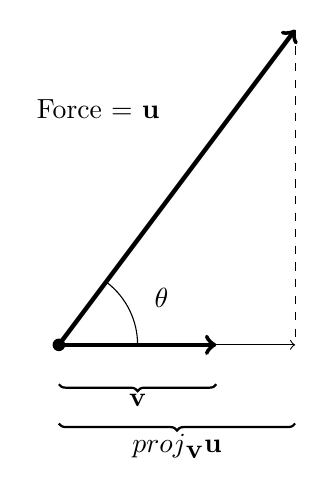
\begin{tikzpicture}
				\fill (0,0) circle (.08);
				\draw[ultra thick,->] (0,0)--(3,4);
				\node at (.5,3) {Force = $\textbf{u}$};
				\draw[dashed] (3,4)--(3,0);
				\draw[->] (0,0)--(3,0);
				\draw[thick,decoration = {brace, mirror, raise = 0.5cm},decorate] (0,0)--(2,0) node[midway, anchor = north, yshift = -.5cm] {$\textbf{v}$};
				\draw[thick,decoration = {brace, mirror, raise = 1cm},decorate] (0,0)--(3,0) node[midway, anchor = north, yshift = -1cm] {$\text{proj}_{\textbf{v}}\textbf{u}$};
				\draw[ultra thick,->] (0,0)--(2,0);
				\draw (1,0) arc (0:52:1) node[pos = 0.7, xshift = .5cm] {$\theta$};
			\end{tikzpicture}
		\end{flushleft}
		
		\begin{ex}
			Let $\textbf{u} = 6\textbf{i} + 3\textbf{j} + 2\textbf{k}$, and $\textbf{v} = \textbf{i} - 2\textbf{j} -2\textbf{k}$.
			\begin{enumerate}[(a)]
				\item Find $\text{proj}_{\textbf{v}}\textbf{u}$.
					\vs{1}
					
				\item Find the scalar projection of $\textbf{u}$ onto $\textbf{v}$.
					\vs{1}
			\end{enumerate}
		\end{ex}
		
		\begin{ex}
			A sled is pulled a distance of 500 m along a horizontal path, by a constant force of 75 N.  The rope attached to the sled forms a $20\dc$ angle with the horizontal; find the work done by the force
		\end{ex}
			\vs{1}
			\newpage
			
	\subsection*{After Class Activities}
		\begin{ex}
			Find the angle between the vectors $\textbf{a} = \lrangle{-2,5}$ and $\textbf{b} = \lrangle{5,12}$
		\end{ex}
			\vs{1}
			
		\begin{ex}
			Are the vectors $\textbf{u} = \lrangle{-5,4,-2}$ and $\textbf{v} = \lrangle{3,4,-1}$ orthogonal, parallel, or neither?
		\end{ex}
			\vs{1}
			
		\begin{ex}
			Find the values of $x$ such that the angle between the vectors $\lrangle{2,1,-1}$ and $\lrangle{1,x,0}$ is $45\dc$.
		\end{ex}
			\vs{1}
			
		\begin{ex}
			If a vector has direction angles $\alpha = \dfrac{\pi}{4}$ and $\beta = \dfrac{\pi}{3}$, find the third direction angle $\gamma$.
		\end{ex}
			\vs{1}
			\newpage
			
		\begin{ex}
			Find the scalar and vector projections of $\textbf{b} = \lrangle{3,-1,1}$ onto $\textbf{a} = \lrangle{4,7,-4}$.
		\end{ex}
			\vs{1}
			
		\begin{ex}
			Show that the vector $\text{orth}_{\textbf{a}}\textbf{b} = \textbf{b} - \text{proj}_{\textbf{a}}\textbf{b}$ is orthogonal to \textbf{a}.  
		\end{ex}
			\vs{1}
			
		\begin{ex}
			Find the work done by a force $\textbf{F} = 8\textbf{i} - 6\textbf{j} + 9\textbf{k}$ that moves an object from the point $(0,10,8)$ to the poitn $(6,12,20)$ along a straight line.  The distance is measured in meters, and the force is measured in newtons.
		\end{ex}
			\vs{2}
\clearpage
\end{document}
